\documentclass[a4paper,12pt]{report}
\usepackage{a4wide}

%\documentclass[a5paper,10pt]{book}
%\usepackage[top=23mm, bottom=18mm, left=15mm, right=25mm]{geometry}
%\geometry{papersize={170mm,220mm}}


\usepackage[utf8x]{inputenc}
\usepackage[danish]{babel}

\usepackage{xr-hyper} %Externe hyper-ref
\usepackage[colorlinks=true, hyperindex=true, linkcolor=minmblaa, citecolor=minmblaa, urlcolor=minmblaa]{hyperref}
\hypersetup{colorlinks=true,filecolor=minmblaa,bookmarksnumbered=true} %Til hyperreferencer. Referencer med farver
\usepackage{needspace} % giver mulighed for at kræve at der skal være et antal tomme linier på siden før ellers indsættes et sideskift.
\usepackage{framed} %Bokse
\usepackage{wrapfig}

\usepackage{amsmath,amsfonts,amssymb,amsthm,mathtools} %Matematikpakker

\setlength{\parindent}{0mm} %Ingen Indhak i første linje i afsnit

\usepackage{color} %Farvepakke

\usepackage{array}
\usepackage{colortbl}
\usepackage{multirow} %Til at flette rækker i tabeller.

\usepackage{verbatim,mhchem}



	% DOWNLOAD FRA: http://sarovar.org/frs/?group_id=52&release_id=97
	% Læg i directory for hoved TEX fil
%\usepackage[draft]{pdfdraftcopy}
%\draftstring{Licens: Kasper Langt Mellemnavn Skårhøj}
%\draftfontsize{30}
	%\draftfontfamily{hlh}
	%\draftangle{45}
	%\definecolor{mycolor}{rgb}{.825,.855,1}
	%\draftcolor{mycolor}
	%\draftfontattrib



% = Sidehoved =
\usepackage{fancyhdr}
\pagestyle{fancy}
\renewcommand{\sectionmark}[1]{\markright{\protect\titlegraphic{dturoed}\textcolor{dtugraa}{\thesection~\MakeUppercase{#1}}}} % \thesection.\
\fancyhead{}
\fancyfoot{}
\fancyhead[R]{\titlefont\thepage}
\fancyhead[C]{}
\fancyhead[L]{\titlefont \small eNote \MakeUppercase{~\thechapter}~\hspace*{1ex}\rightmark}
\renewcommand\headrulewidth{0pt}
\fancypagestyle{plain}{\fancyfoot[C]{}}% {\titlefont\footnotesize\thepage}}
\setlength{\headheight}{15pt}


% = Længder
%\newlength{\envtblsep}\setlength{\envtblsep}{1\FrameSep}
\newlength{\obsl}\setlength{\obsl}{\textwidth-1.2cm-13.2pt}

% Includes:

% =     Fonts (select one)    =
\usepackage{mathpazo}\linespread{1.05} % Palatino needs more leading (space between lines)
\usepackage{bm} % bold math, must be loaded after the fontpackages

% % Til overskrifter
\DeclareTextFontCommand{\th}{\fontencoding{T1}\fontfamily{phv}\fontseries{b}\selectfont}
\newcommand\titlefont{\fontencoding{T1}\fontfamily{phv}\selectfont}


% =     PGF grafik      =
\usepackage{tikz}
\newcommand\titlegraphic[1]{%
\tikz[baseline] %
\draw[thick,color=#1]
(0pt  ,-0.25em) -- (0pt  ,0.85em)
(2.5pt,-0.25em) -- (2.5pt,0.85em)
(5pt  ,-0.25em) -- (5pt  ,0.85em)
(7.5pt,-0.25em) -- (7.5pt,0.85em);\hspace*{0.8ex} %
}

\newcommand\titlegraphicwide[1]{%
\tikz[baseline] %
\draw[line width=0.8mm,color=#1]
(0pt  ,-0.25em) -- (0pt  ,0.85em)
(4.5pt,-0.25em) -- (4.5pt,0.85em)
(9pt  ,-0.25em) -- (9pt  ,0.85em)
(13.5pt,-0.25em) -- (13.5pt,0.85em);\hspace*{0.8ex} %
}


% =      Title Layout      =
\usepackage{titlesec}
\makeatletter
\titleformat{\chapter}
	[display] % Shape
	{\titlefont\Huge\flushleft} % Title and label format
	{\titlefont\LARGE\bfseries \titlegraphicwide{dturoed}\textcolor{dtugraa}{\@chapapp~\thechapter}} % label
	{0.9em} % label/title separation
	{} % before code
	[] % after code
\makeatother
\titleformat{\section}
	[hang] % Shape
	{\titlefont\Large\flushleft} % Title and label format
	{\thesection} % label
	{0.9em} % label/title separation
	{} % before code
	[] % after code
\titleformat{\subsection}
	[hang] % Shape
	{\titlefont\large} % Title and label format
	{\thesubsection} % label
	{0.9em} % label/title separation
	{} % before code
	[] % after code
\titlespacing{\subsection}{0pt}{*6}{*1.5}
\titleformat{\subsubsection}
	[hang] % Shape
	{\titlefont} % Title and label format
	{\thesubsubsection} % label
	{0.9em} % label/title separation
	{} % before code
	[] % after code



% = Farver
\definecolor{dturoed}{rgb}{0.6, 0.0, 0.0}
\definecolor{dtugraa}{rgb}{0.5, 0.5, 0.5}	% Lidt mørkere. Korrekt = 0.4
\definecolor{mingroenstreg}{rgb}{0.4,0.8,0}	% Sekundærfarve 14 : 102/204/0	(Forårsgrøn) -> Eksempler
\definecolor{mingroen}{rgb}{0.32,0.64,0}		% Sekundærfarve 14, 80% mørkere (tekst)
\definecolor{minorangestreg}{rgb}{1,0.6,0}		% Sekundærfarve 1 : 255/153/0	(Orange) -> Opgaver
\definecolor{minorange}{rgb}{0.8,0.48,0}		% Sekundærfarve 1 , 80% mørkere (tekst)

\definecolor{minblaa}{rgb}{0.2,0.4,0.8}	% Sekundærfarve 13 , 51/102/204 	( Blå -> Definitioner etc)
\definecolor{minmblaa}{rgb}{0.16,0.32,0.64}	% Sekundærfarve 13 , 80% mørkere (tekst)
\definecolor{thmbackground}{rgb}{0.97,.97, 0.99}	% Farve 13 - lys baggrund

\definecolor{mingraastreg}{rgb}{.5,.5,.5}
\definecolor{hvadbackground}{rgb}{0.97,.97, 0.97}
\definecolor{sumgul}{rgb}{1,1,.8}

\definecolor{hjmopgfarve}{rgb}{.96,1,.96}


% = Counter
\newcounter{evncount}[chapter]
\setcounter{evncount}{0}
\renewcommand{\theevncount}{\thechapter.\arabic{evncount}}
\renewcommand{\theequation}{\thechapter-\arabic{equation}}


% = Eksempler = example =
\newenvironment{example}[1][]{
	\refstepcounter{evncount}
	\setlength{\obsl}{\textwidth-1.2cm-13.2pt-9pt} % fix width of the info envirnment%
	\def\FrameCommand{ 
		\textcolor{mingroenstreg}{\vrule width 4pt} 
		\hspace{5pt} 
	}%
	\MakeFramed{\advance\hsize-\width \FrameRestore}%
	\needspace{3\baselineskip}
	\titlegraphic{mingroen}
	\textcolor{mingroen}{
		\th{Eksempel \theevncount \hspace*{5mm} #1}
	} 
	\vspace*{3mm}%
	\begin{small}
	\par
}
{
	\end{small}
	\endMakeFramed
}


% = Opgaver = exercise =
\newenvironment{exercise}[1][]{
	\refstepcounter{evncount}
	\setlength{\obsl}{\textwidth-1.2cm-13.2pt-9pt}% fix width of the info envirnment%
	\def\FrameCommand{
		\textcolor{minorangestreg}{\vrule width 4pt}
		\hspace{5pt}
	}%
	\MakeFramed{\advance\hsize-\width \FrameRestore}%
	\needspace{3\baselineskip}
	\titlegraphic{minorange}
	\textcolor{minorange}{
		\th{Opgave \theevncount \hspace*{5mm} #1}
	} 
	\vspace*{3mm}%
	\begin{small}
	\par
}
{
	\end{small}
	\endMakeFramed
}


% = Bevis
\newenvironment{bevis}{
	\setlength{\obsl}{\textwidth-1.2cm-13.2pt-9pt} % fix width of the info envirnment%
	\def\FrameCommand{
		\textcolor{mingraastreg}{\vrule width 4pt} 
		\hspace{5pt}
	}%
	\MakeFramed{\advance\hsize-\width \FrameRestore}%
	\needspace{3\baselineskip}
	\titlegraphic{black}
	\textcolor{black}{
		\th{Bevis}
	}
	\vspace*{3mm}%
	\begin{small}
	\par
}
{
	\bevisslut 
	\end{small}
	\endMakeFramed
}


% = Definition =
\newenvironment{definition}[1][]{
	\vspace{4mm}
	\pagebreak[1]
	\setlength{\obsl}{\textwidth-1.2cm-2\FrameSep-13.2pt}%
	\def\FrameCommand{
		\fboxsep=\FrameSep\fcolorbox{minblaa}{thmbackground}
	}
	\begin{minipage}{\textwidth}
	\MakeFramed{\advance\hsize-\width\FrameRestore}
	\refstepcounter{evncount}
	\titlegraphic{minblaa}
	\textcolor{minmblaa}{
		\th{Definition \theevncount \hspace*{5mm} #1}
	}
	\vspace*{3mm}
	\par
}
{
	\endMakeFramed 
	\end{minipage}
	\vspace{4mm}
}


% = Theorem =
\newenvironment{theorem}[1][]{
	\vspace{4mm}
	\pagebreak[1]%
	\setlength{\obsl}{\textwidth-1.2cm-2\FrameSep-13.2pt}%
	\def\FrameCommand{
		\fboxsep=\FrameSep\fcolorbox{minblaa}{thmbackground}
	}%
	\begin{minipage}{\textwidth}
	\MakeFramed{\advance\hsize-\width\FrameRestore}%
	\refstepcounter{evncount}
	\titlegraphic{minblaa}
	\textcolor{minmblaa}{
		\th{Sætning \theevncount \hspace*{5mm} #1}
	}
	\vspace*{3mm}
	\par
}
{
	\endMakeFramed 
	\end{minipage}
	\vspace{4mm}
}


% = Lemma =
\newenvironment{lemma}[1][]{
	\vspace{4mm}
	\pagebreak[1]
	\setlength{\obsl}{\textwidth-1.2cm-2\FrameSep-13.2pt}%
	\def\FrameCommand{
		\fboxsep=\FrameSep \fcolorbox{minblaa}{thmbackground}
	}
	\begin{minipage}{\textwidth} 
	\MakeFramed{\advance\hsize-\width \FrameRestore}
	\refstepcounter{evncount}
	\titlegraphic{minblaa}
	\textcolor{minmblaa}{
		\th{Hjælpesætning \theevncount \hspace*{5mm} #1}
	}
	\vspace*{3mm}
	\par
}
{
	\endMakeFramed 
	\end{minipage}
	\vspace{4mm}
}


% = Corollary =
\newenvironment{corollary}[1][]{
	\vspace{4mm}
	\pagebreak[1]
	\setlength{\obsl}{\textwidth-1.2cm-2\FrameSep-13.2pt}%
	\def\FrameCommand{
		\fboxsep=\FrameSep \fcolorbox{minblaa}{thmbackground}
	}
	\begin{minipage}{\textwidth} 
	\MakeFramed{\advance\hsize-\width \FrameRestore}
	\refstepcounter{evncount}
	\titlegraphic{minblaa}
	\textcolor{minmblaa}{
		\th{Følgesætning \theevncount \hspace*{5mm} #1}
	}
	\vspace*{3mm}
	\par
}
{
	\endMakeFramed 
	\end{minipage}
	\vspace{4mm}
}


% = Metode = method
\newenvironment{method}[1][]{
	\vspace{4mm}
	\pagebreak[1]
	\setlength{\obsl}{\textwidth-1.2cm-2\FrameSep-13.2pt}%
	\def\FrameCommand{
		\fboxsep=\FrameSep \fcolorbox{black}{hvadbackground}
	}
	\begin{minipage}{\textwidth} 
	\MakeFramed{\advance\hsize-\width \FrameRestore}
	\refstepcounter{evncount}
	\titlegraphic{black}
	\textcolor{black}{
		\th{Metode \theevncount \hspace*{5mm} #1}
	}
	\vspace*{3mm}
	\par
}
{
	\endMakeFramed
	\end{minipage}
	\vspace{4mm}
}


% = Forklaring = explain =
\newenvironment{explain}[1][]{
	\vspace{4mm}
	\pagebreak[1]
	\setlength{\obsl}{\textwidth-1.2cm-2\FrameSep-13.2pt}%
	\def\FrameCommand{
		\fboxsep=\FrameSep \fcolorbox{black}{hvadbackground}
	}
	\MakeFramed{\advance\hsize-\width \FrameRestore}
	\refstepcounter{evncount}
	\titlegraphic{black}
	\textcolor{black}{
		\th{Forklaring \theevncount \hspace*{5mm} #1}
	}
	\vspace*{3mm}
	\par
}
{
	\endMakeFramed
	\vspace{4mm}
}


% = Bemærkning = remark =
\newenvironment{remark}[1][]{
	\vspace{4mm}
	\pagebreak[1]
	\setlength{\obsl}{\textwidth-1.2cm-2\FrameSep-13.2pt}%
	\def\FrameCommand{
		\fboxsep=\FrameSep \fcolorbox{black}{hvadbackground}
	}
	\begin{minipage}{\textwidth} 
	\MakeFramed{\advance\hsize-\width \FrameRestore}
	\refstepcounter{evncount}
	\titlegraphic{black}
	\textcolor{black}{
		\th{Bemærkning \theevncount \hspace*{5mm} #1}
	}
	\vspace*{3mm}
	\par
}
{
	\endMakeFramed 
	\end{minipage}
	\vspace{4mm}
}







% = OBS! = obs =
\newenvironment{obs}{\vspace{4mm}\par%
\begin{tabular}{m{1.2cm}<{\hspace*{2mm}}@{}|m{\obsl}@{}}\hspace*{-4pt}\raggedleft
\includegraphics[width=1.1cm]{../Strukturfiler/FIGS/Alert01} & \begin{minipage}{\obsl}}{\end{minipage}\\ \end{tabular}\vspace{4mm}\par}


% = INFO = info =
\newenvironment{info}{\vspace{4mm}\par%
\begin{tabular}{m{1.2cm}<{\hspace*{2mm}}@{}|m{\obsl}@{}}\hspace*{-4pt}\raggedleft
\includegraphics[width=1.1cm]{../Strukturfiler/FIGS/Info01} & \begin{minipage}{\obsl}}{\end{minipage}\\ \end{tabular}\vspace{4mm}\par}


% = THINK= think =
\newenvironment{think}{\vspace{4mm}\par%
\begin{tabular}{m{1.2cm}<{\hspace*{2mm}}@{}|m{\obsl}@{}}\hspace*{-4pt}\raggedleft
\includegraphics[width=0.7cm]{../Strukturfiler/FIGS/ChessPiece} & \begin{minipage}{\obsl}}{\end{minipage}\\ \end{tabular}\vspace{4mm}\par}


% = AHA= aha =
\newenvironment{aha}{\vspace{4mm}\par%
\begin{tabular}{m{1.2cm}<{\hspace*{2mm}}@{}|m{\obsl}@{}}\hspace*{-4pt}\raggedleft
\includegraphics[width=1.1cm]{../Strukturfiler/FIGS/Think} & \begin{minipage}{\obsl}}{\end{minipage}\\ \end{tabular}\vspace{4mm}\par}


% = BUILDUP= build =
\newenvironment{build}{\vspace{4mm}\par%
\begin{tabular}{m{1.2cm}<{\hspace*{2mm}}@{}|m{\obsl}@{}}\hspace*{-4pt}\raggedleft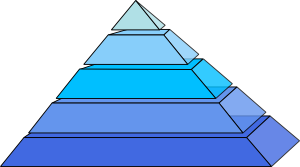
\includegraphics[width=1.1cm]{../Strukturfiler/FIGS/BluePyramid} & \begin{minipage}{\obsl}}{\end{minipage}\\ \end{tabular}\vspace{4mm}\newline}


% = Forudsætning = basis
\newenvironment{basis}{\begin{flushleft} \begin{itshape} }{\end{itshape} \end{flushleft}}


% = Opsummering =
\newenvironment{summary}{\clearpage\pagecolor{sumgul}\section{Opsummering}}{\newpage\pagecolor{white}}











% = Counter
\newcounter{opgavecount}[section]
\setcounter{opgavecount}{0}
\newcounter{spgcount}[opgavecount]
\setcounter{spgcount}{0}
\renewcommand{\thespgcount}{\alph{spgcount})}



% = EXERCISE = (DIVIDER)

\newcommand{\exercisebegin}[1][]{\bigskip\needspace{3\baselineskip}\refstepcounter{opgavecount}\titlegraphic{mingroen}\textcolor{mingroen}{\th{Opgave \theopgavecount \hspace*{1cm} #1}}\medskip\par}

% = QUIZEXERCISE = (DIVIDER)

\newcommand{\quizexercisebegin}[1][]{\bigskip\needspace{3\baselineskip}\refstepcounter{opgavecount}\titlegraphic{mingroen}\textcolor{mingroen}{\th{Quiz-Opgave \theopgavecount \hspace*{1cm} #1}}\medskip\par}

% = QUESTION =

\newenvironment{question}{\refstepcounter{spgcount}\begin{itemize}\item[\thespgcount]}{\end{itemize}\hspace*{\fill}}

% = VINK =

\newenvironment{vink}{\begin{tabular}{m{.9cm}<{\hspace*{2mm}}@{}|m{\obsl}@{}}\hspace*{-4pt}\raggedleft
\includegraphics[width=.9cm]{../Strukturfiler/FIGS/Think} & \begin{minipage}{\obsl}}{\end{minipage}\\ \end{tabular}\medskip\\}
	
% = FACIT =

\newenvironment{facit}{\begin{tabular}{m{.9cm}<{\hspace*{2mm}}@{}|m{\obsl}@{}}\hspace*{-4pt}\raggedleft
\includegraphics[width=.9cm]{../Strukturfiler/FIGS/Check} & \begin{minipage}{\obsl}}{\end{minipage}\\ \end{tabular}\medskip\\}








\newcommand{\afsnit}[1]{\bigskip\th{\titlegraphic{mingroen}\textcolor{mingroen}{#1}} \\ \rule[7pt]{.4\textwidth}{1pt} \vspace*{-2.5mm}\par}

% (DIVIDER):
\newcommand{\ugedagdatotitel}[4]{\pagebreak[4]\section{Semesteruge #1 -- #2 Dag \hspace*{1mm} (#3)} \vspace*{-4mm} \rule[5pt]{\textwidth}{1pt}\vspace*{-2.5mm} \begin{center}\large{\th{#4}}\end{center} \fancyhead[C]{\th{Semesteruge #1}}}

\newenvironment{skema}[1]{\definecolor{shadecolor}{rgb}{0.96,.98, 1.0} \setlength{\FrameSep}{6pt} \renewcommand{\FrameHeightAdjust}{10pt} \vspace*{-4pt}\begin{shaded} \begin{tabular}{#1}}{\end{tabular} \end{shaded} \vspace*{-7pt}}


% ========================

% MAKROER

%\newenvironment{matr}[1][]{\hspace*{-.8mm}\left[\hspace*{-1mm}\begin{array}{#1}}{\end{array}\hspace*{-1mm}\right]\hspace*{-.8mm}}
\newcommand{\bevisslut}{\begin{scriptsize} \begin{flushright} $ \blacksquare $ \end{flushright} \end{scriptsize}}

\newcommand{\tref}[2]{\hyperref[#1]{#2 \ref*{#1}}}
\newcommand{\thref}[2]{\hyperref[#1]{#2}}

\newcommand{\refA}[1]{\colorbox{yellow}{\ref{#1}}}
\newcommand{\hrefA}[2]{\colorbox{yellow}{\href{#1}{#2}}}
\newcommand{\trefA}[2]{\colorbox{yellow}{\hyperref[#1]{#2 \ref*{#1}}}}
\newcommand{\threfA}[2]{\colorbox{yellow}{\hyperref[#1]{#2}}}

\newenvironment{matr}[1]{\hspace*{-.8mm}\begin{bmatrix}\hspace*{-1mm}\begin{array}{#1}}{\end{array}\hspace*{-1mm}\end{bmatrix}\hspace*{-.8mm}}
\newcommand{\transp}{\hspace*{-.6mm}^{\top}}

\newcommand{\maengde}[2]{\left\lbrace \hspace*{-1mm} \begin{array}{c|c} #1 & #2 \end{array} \hspace*{-1mm} \right\rbrace}

\newenvironment{eqnalign}[1]{\setlength{\arraycolsep}{1.3pt}\begin{equation}\begin{array}{#1}}{\end{array}\end{equation}\par}
\newcommand{\eqnl}{\setlength{\arraycolsep}{1.3pt}}

\newcommand{\matind}[3]{{_\mathrm{#1}\mathbf{#2}_\mathrm{#3}}}
\newcommand{\vekind}[2]{{_\mathrm{#1}\mathbf{#2}}}
\newcommand{\jac}[2]{{\mathrm{Jacobi}_\mathbf{#1} (#2)}}
\newcommand{\diver}[2]{{\mathrm{div}\mathbf{#1} (#2)}}
\newcommand{\rot}[1]{{\mathbf{rot}\mathbf{(#1)}}}

\newcommand{\am}{\mathrm{am}}
\newcommand{\gm}{\mathrm{gm}}
\newcommand{\E}{\mathrm{E}}
\newcommand{\Span}{\mathrm{span}}
\newcommand{\mU}{\mathbf{U}}

\newcommand{\ms}{\medskip\\}
\newcommand{\bs}{\bigskip\\}

\newcommand{\mA}{\mathbf{A}}
\newcommand{\mB}{\mathbf{B}}
\newcommand{\mC}{\mathbf{C}}
\newcommand{\mD}{\mathbf{D}}
\newcommand{\mE}{\mathbf{E}}
\newcommand{\mF}{\mathbf{F}}
\newcommand{\mK}{\mathbf{K}}
\newcommand{\mI}{\mathbf{I}}
\newcommand{\mM}{\mathbf{M}}
\newcommand{\mN}{\mathbf{N}}
\newcommand{\mQ}{\mathbf{Q}}
\newcommand{\mT}{\mathbf{T}}
\newcommand{\mV}{\mathbf{V}}
\newcommand{\mW}{\mathbf{W}}
\newcommand{\mX}{\mathbf{X}}
\newcommand{\ma}{\mathbf{a}}
\newcommand{\mb}{\mathbf{b}}
\newcommand{\mc}{\mathbf{c}}
\newcommand{\md}{\mathbf{d}}
\newcommand{\me}{\mathbf{e}}
\newcommand{\mn}{\mathbf{n}}
\newcommand{\mr}{\mathbf{r}}
\newcommand{\mv}{\mathbf{v}}
\newcommand{\mw}{\mathbf{w}}
\newcommand{\mx}{\mathbf{x}}
\newcommand{\mxb}{\mathbf{x_{bet}}}
\newcommand{\my}{\mathbf{y}}
\newcommand{\mz}{\mathbf{z}}
\newcommand{\reel}{\mathbb{R}}
\newcommand{\mL}{\bm{\Lambda}} %Lambda-matrix
\newcommand{\mnul}{\bm{0}}
\newcommand{\trap}[1]{\mathrm{trap}(#1)}
\newcommand{\Det}{\operatorname{Det}}
\newcommand{\adj}{\operatorname{adj}}
\newcommand{\Ar}{\operatorname{Areal}}
\newcommand{\Vol}{\operatorname{Vol}}
\newcommand{\Rum}{\operatorname{Rum}}
\newcommand{\diag}{\operatorname{\bf{diag}}}
\newcommand{\bidiag}{\operatorname{\bf{bidiag}}}
\newcommand{\spanVec}[1]{\mathrm{span}\{#1\}}
\newcommand{\Div}{\operatorname{Div}}
\newcommand{\Rot}{\operatorname{\mathbf{Rot}}}

\newcommand{\Jac}{\operatorname{Jacobi}}
\newcommand{\Tan}{\operatorname{Tan}}
\newcommand{\Ort}{\operatorname{Ort}}
\newcommand{\Flux}{\operatorname{Flux}}
\newcommand{\Cmass}{\operatorname{Cm}}
\newcommand{\Imom}{\operatorname{Im}}
\newcommand{\Pmom}{\operatorname{Pm}}
\newcommand{\IS}{\operatorname{I}}
\newcommand{\IIS}{\operatorname{II}}
\newcommand{\IIIS}{\operatorname{III}}
\newcommand{\Le}{\operatorname{L}}
\newcommand{\app}{\operatorname{app}}
\newcommand{\M}{\operatorname{M}}
\newcommand{\re}{\mathrm{Re}}
\newcommand{\im}{\mathrm{Im}}

\newcommand{\compl}{\mathbb{C}} %de komplekse tal
\newcommand{\e}{\mathrm{e}} %eksponentialfunktionen. lodret 'e', og altså ikke kursiv ligesom andre bogstaver.





% Medialink: SCREEN: (QRcode) + thumbnail image + link på kodenummer (til qr.dtu.dk)
\newcommand{\onlinemedia}[3]{
	\begin{wrapfigure}{r}{3.2cm} 
		\vspace{-30pt} 
		\vspace{#1pt} 
		\begin{flushright} 
			\includegraphics[width=3cm]{qr/#2.png} 
			\tiny 
			\href{http://qr.dtu.dk/#2}{#2: #3}
			\normalsize  
		\end{flushright} 
		\vspace{-10pt} 
	\end{wrapfigure}
}
\newcommand{\onlinemediathumb}[3]{
	\begin{wrapfigure}{r}{3.2cm} 
		\vspace{-30pt} 
		\vspace{#1pt} 
		\begin{flushright} 
			\includegraphics[width=3cm]{qr/#2.png} 
			\includegraphics[width=3cm]{qr/#2_thumb.png} 
			\tiny 
			\href{http://qr.dtu.dk/#2}{#2: #3}
			\normalsize  
		\end{flushright} 
		\vspace{-10pt} 
	\end{wrapfigure}
}



% Index:
\usepackage{makeidx}
\makeindex
\newcommand\ind[2]{\index{#1}\textbf{\textit{\textcolor{black}{#2}}}}

% ###SERVER_EXCLUDE_BEGIN###
\externaldocument[NUID17-]{../../enoten/TN01-Talrum/Talrum}
\externaldocument[NUID1-]{../../enoten/TN02-Ligningssystemer/TNdriver}
\externaldocument[NUID2-]{../../enoten/TN03-Matricer_og_Matrixalgebra/Matricer_og_matrixalgebra}
\externaldocument[NUID3-]{../../enoten/TN04-Kvadratiske_matricer/TNdriver}
\externaldocument[NUID11-]{../../enoten/TN05-Determinanter/Determinanter}
\externaldocument[NUID12-]{../../enoten/TN06-GeometriskeVektorer/GeometriskeVektorer}
\externaldocument[NUID18-]{../../enoten/TN07-Vektorrum/VektorRum}
\externaldocument[NUID21-]{../../enoten/TN08-LinAfbildninger/LinAfbildninger}
\externaldocument[NUID23-]{../../enoten/TN09-Egenvaerdier_og_egenvektorer/TNdriver}
\externaldocument[NUID24-]{../../enoten/TN10-Diagonalisering_med_egenvektorer/TNdriver}
\externaldocument[NUID10-]{../../enoten/TN11-1.ordens_differentialligninger/TNdriver}
\externaldocument[NUID13-]{../../enoten/TN12-1.ordens_differentialligningssystemer/TNdriver}
\externaldocument[NUID14-]{../../enoten/TN13-2.ordens_differentialligninger/TNdriver}
\externaldocument[NUID27-]{../../enoten/TN14-Elemenataere_funktioner/Elementaere_Funktioner}
\externaldocument[NUID28-]{../../enoten/TN15-Funktioner2Variable/Funktioner_To_Variable}
\externaldocument[NUID29-]{../../enoten/TN16-Gradienter_og_Tangentplaner/Gradienter_og_Tangentplaner}
\externaldocument[NUID32-]{../../enoten/TN17-Taylor_formler/Taylor_Formler}
\externaldocument[NUID33-]{../../enoten/TN18-Taylor_2Var/Taylor_2Var}
\externaldocument[NUID34-]{../../enoten/TN19-SymMat/SymmetriskeMatricer}
\externaldocument[NUID35-]{../../enoten/TN20-KegleSnit/Keglesnit}
\externaldocument[NUID36-]{../../enoten/TN21-Riemann_Integral/Riemann_01}
\externaldocument[NUID37-]{../../enoten/TN22-Plan_Int/Plan_Int_01}
\externaldocument[NUID39-]{../../enoten/TN23-Flade_Int/Flade_Rum_Int_01}
\externaldocument[NUID40-]{../../enoten/TN24-Vektorfelter/Vektorfelter_01}
\externaldocument[NUID41-]{../../enoten/TN25-Flux/Flux_02}
\externaldocument[NUID42-]{../../enoten/TN26-Gauss/Gauss_01}
\externaldocument[NUID128-]{../../enoten/TN27-Stokes/Stokes_01}
\externaldocument[NUID43-]{../../enoten/TN29-KomplekseTal/KomplekseTal}

\externaldocument[NUID6-]{../../E-math-opgaver/Opgaver/opgU123}
\externaldocument[NUID19-]{../../E-math-opgaver/Opgaver/opgU45}
\externaldocument[NUID20-]{../../E-math-opgaver/Opgaver/opgU678}
\externaldocument[NUID25-]{../../E-math-opgaver/Opgaver/opgU910SD}
\externaldocument[NUID31-]{../../E-math-opgaver/OpgaverF11-U123/opgF123}
% \externaldocument[NUID9-]{../../E-math-opgaver/Opgaver/Dagsordner E10}
% ###SERVER_EXCLUDE_END###


% Begin document and set alternative chapter title:
\begin{document}
\renewcommand{\chaptername}{eNote}

\setcounter{chapter}{2}

\chapter{Matricer og Matrixalgebra} \label{tn3}

\begin{basis}
Denne eNote introducerer matricer og regneoperationer for matricer, og udvikler hertil hørende regneregler. Noten kan læses uden andet grundlag end gymnasiet, men det kan være en idé, at være bekendt med talrummet $ \reel^n $, som beskrives i \tref{NUID17-tn1}{eNote}.
\end{basis}

En \ind{matrix}{matrix} er en form for talskema. Her er et eksempel på en matrix kaldet $ \mM $:
\begin{equation}
\mM = \begin{matr}{rrr} 1 & 4 & 3 \\ -1 & 2 & 7 \end{matr}
\end{equation}
En matrix karakteriseres ved antallet af \textit{rækker} og \textit{søjler}, og matricen $ \mM $ kaldes derfor en $ 2 \times 3 $ matrix. Matricen $ \mM $ siges at indeholde $ 2 \cdot 3 = 6 $ \textit{elementer}. Udover rækker, søjler og elementer har matricer en række andre begreber tilknyttet. For at beskrive dem opstilles en generel matrix, her kaldet $ \mA $:
\begin{equation}
\mA = \begin{matr}{cccc} a_{11} & a_{12} & \ldots & a_{1n} \\ a_{21} & a_{22} & \ldots & a_{2n} \\ \vdots & \vdots & & \vdots \\ a_{m1} & a_{m2} & \ldots & a_{mn} \end{matr}
\end{equation}
Matricen $ \mA $ har således $ m $ rækker og $ n $ søjler, og man kan ligeledes skrive $ \mA_{m \times n} $ eller $ m \times n $ \textit{matricen} $ \mA $. Matricen $ \mA $ siges også at være \textit{af typen} $ m \times n $. \bs
To $ m \times n $-matricer  $ \mA $ og $\mB$ kaldes \textit{ens} hvis de elementvis er ens, og man skriver da $\,\mA =\mB\,$.\bs
En matrix, som kun har én søjle ($ n = 1 $), kaldes en \textit{søjlematrix}. Tilsvarende kaldes en matrix med kun én række ($ m = 1 $) en \textit{rækkematrix}. \bs
En matrix med lige mange rækker og søjler ($ m = n $), kaldes en \textit{kvadratisk matrix}. Kvadratiske matricer underkastes særlig undersøgelse i \tref{NUID3-tn4}{eNote}. \bs
Er alle elementerne i en $n\times n$-matrix reelle tal, kaldes matricen for en \textit{reel matrix}. Mængden af disse matricer betegnes $ \reel^{m \times n} $. \bs
Matricen, hvis alle elementer er lig med 0, kaldes \textit{nulmatricen} uanset type, og betegnes $ \mnul $ eller evt. $ \mnul_{m \times n} $. Enhver anden matrix kaldes en \textit{egentlig matrix}.

\section{Matrixsum og produkt af matrix med skalar}

Det er muligt at lægge to matricer sammen, hvis de er af samme type. Man lægger da elementerne sammen pladsvis og danner derved en ny matrix af samme type. Ligeså kan man gange en matrix med en skalar (et tal), det sker ved at gange alle elementerne med skalaren.

\begin{definition}[Matrixsum og produkt med skalar] \label{tn3.sum}
Givet er en skalar $ k \in \reel $ og to reelle matricer $ \mA_{m \times n} $ og $ \mB_{m \times n} $:
\begin{equation}
\mA = \begin{matr}{cccc} a_{11} & a_{12} & \ldots & a_{1n} \\ a_{21} & a_{22} & \ldots & a_{2n} \\ \vdots & \vdots & & \vdots \\ a_{m1} & a_{m2} & \ldots & a_{mn} \end{matr}
\quad \mathrm{og} \quad
\mB = \begin{matr}{cccc} b_{11} & b_{12} & \ldots & b_{1n} \\ b_{21} & b_{22} & \ldots & b_{2n} \\ \vdots & \vdots & & \vdots \\ b_{m1} & b_{m2} & \ldots & b_{mn} \end{matr}
\end{equation}
\textit{Summen} af matricerne defineres således:
\begin{equation}
\mA + \mB = \begin{matr}{cccc} a_{11} + b_{11} & a_{12} + b_{12} & \ldots & a_{1n} + b_{1n} \\ a_{21} + b_{21} & a_{22} + b_{22} & \ldots & a_{2n} + b_{2n} \\ \vdots & \vdots & & \vdots \\ a_{m1} + b_{m1} & a_{m2} + b_{m2} & \ldots & a_{mn} + b_{mn} \end{matr}
\end{equation}
Summen er kun defineret, når matricerne er af samme type. \bs
\textit{Produktet} af matricen $ \mA $ med skalaren $ k $ skrives $ k \mA $ eller $ \mA k$ og defineres således:
\begin{equation}
k \mA = \mA k = \begin{matr}{cccc} k \cdot a_{11} & k \cdot a_{12} & \ldots & k \cdot a_{1n} \\ k \cdot a_{21} & k \cdot a_{22} & \ldots & k \cdot a_{2n} \\ \vdots & \vdots & & \vdots \\ k \cdot a_{m1} & k \cdot a_{m2} & \ldots & k \cdot a_{mn} \end{matr}
\end{equation}
\end{definition}

Den \textit{modsatte vektor} $-\mA\,$ til en matrix $\mA$ defineres som den matrix der fremkommer ved at alle elementerne i $\mA$ ganges med $-1\,$. Det ses at $-\mA=(-1)\mA\,$.\bs
\begin{example}[Simple matrixoperationer] \label{eks.simpleop}
Der er givet to matricer $ \mA $ og $ \mB $ ved:
\begin{equation}
\mA = \begin{matr}{rr} 4 & -1 \\ 8 & 0 \end{matr}
\quad \mathrm{og} \quad
\mB = \begin{matr}{rr} -4 & 3 \\ 9 & \tfrac{1}{2} \end{matr}
\end{equation}
Matricerne er begge af typen $ 2 \times 2 $. Vi ønsker at bestemme en tredje og fjerde matrix $ \mC = 4\mA $ og $ \mD~=~2\mA + \mB $. Dette kan gøres ved hjælp af definition \ref{tn3.sum}.
\begin{equation}
\begin{aligned}
\mC &= 4\mA = 4 \cdot \begin{matr}{rr} 4 & -1 \\ 8 & 0 \end{matr} = \begin{matr}{cc} 4 \cdot 4 & 4 \cdot (-1) \\ 4 \cdot 8 & 4 \cdot 0 \end{matr} = \begin{matr}{rr} 16 & -4 \\ 32 & 0 \end{matr} \\
\mD &= 2\mA + \mB = \begin{matr}{rr} 8 & -2 \\ 16 & 0 \end{matr} + \begin{matr}{rr} -4 & 3 \\ 9 & +\tfrac{1}{2} \end{matr} = \begin{matr}{rr} 4 & 1 \\ 25 & \tfrac{1}{2} \end{matr}
\end{aligned}
\end{equation}
\end{example}

I følgende sætning opsummeres de regneregler, der gælder for sum af matricer og produkt med skalar.

\begin{theorem}[Regneregler for matrixsum og produkt med skalar] \label{tn3.regneregler}
For vilkårlige matricer $ \mA $, $ \mB $ og $ \mC $ i $ \reel^{m \times n} $ og ligeledes vilkårlige reelle tal $ k_1 $ og $ k_2 $ gælder følgende regneregler: \smallskip \\
\begin{tabular}{lcl}
1. & $ \mA + \mB = \mB + \mA $ & Addition er kommutativ \smallskip \\
2. & $ (\mA + \mB) + \mC = \mA + (\mB + \mC) $ & Addition er associativ \smallskip \\
3. & $ \mA + \mnul = \mA $ & $ \mnul $ er en neutral matrix for addition i $ \reel^{m \times n} $ \smallskip  \\
4. & $ \mA + (-\mA) = \mnul $ & Alle matricer i $ \reel^{m \times n} $ har en modsat matrix \smallskip \\
5. & $ k_1(k_2\mA) = (k_1k_2)\mA $ & Produkt af matrix med skalarer er associativ \smallskip \\
6. & $ (k_1 + k_2)\mA = k_1\mA + k_2\mA $ & \multirow{2}{10cm}{$\biggr\rbrace$ De distributive regler gælder} \smallskip \\
7. & $ k_1(\mA+\mB) = k_1\mA + k_1\mB $ &  \smallskip  \\
8. & $ 1\mA = \mA $ & Skalaren $ 1 $ er neutral i produkt med matrix \\
\end{tabular}
\end{theorem}

Regnereglerne i sætning \ref{tn3.regneregler} kan vises ved hjælp af sædvanlige regneregler for reelle tal. Fremgangsmåden eksempliceres for to af regnereglernes vedkommende i det følgende eksempel.

\begin{example}[Eftervisning af regneregel] \label{tn3.regnereglereks}
Givet er de to matricer
\begin{equation}
\mA = \begin{matr}{cc} a_{11} & a_{12} \\ a_{21} & a_{22} \end{matr} \quad \mathrm{og} \quad \mB = \begin{matr}{cc} b_{11} & b_{12} \\ b_{21} & b_{22} \end{matr}
\end{equation}
samt konstanterne $ k_1 $ og $ k_2 $. Vi prøver nu som eksempel at eftervise de distributive regler, som står i sætning \ref{tn3.regneregler}. Først haves:
\begin{equation}
\begin{aligned}
(k_1 + k_2)\mA &= (k_1 + k_2) \begin{matr}{cc} a_{11} & a_{12} \\ a_{21} & a_{22} \end{matr} = \begin{matr}{cc} (k_1 + k_2)a_{11} & (k_1 + k_2)a_{12} \\ (k_1 + k_2)a_{21} & (k_1 + k_2)a_{22} \end{matr} \\
k_1\mA + k_2\mA &= \begin{matr}{cc} k_1a_{11} & k_1a_{12} \\ k_1a_{21} & k_1a_{22} \end{matr} + \begin{matr}{cc} k_2a_{11} & k_2a_{12} \\ k_2a_{21} & k_2a_{22} \end{matr} = \begin{matr}{cc} k_1a_{11} + k_2a_{11} & k_1a_{12} + k_2a_{12} \\ k_1a_{21} + k_2a_{21} & k_1a_{22} + k_2a_{22} \end{matr}
\end{aligned}
\end{equation}
Sættes $ a_{11},a_{12},a_{21} $ og $ a_{22} $ uden for parentes i hvert af elementerne i det sidste udtryk, ses det at $ (k_1 + k_2)\mA = k_1\mA + k_2\mA $ i dette tilfælde. Det at sætte $ a $-elementerne uden for parentes er netop at bruge den distributive regel for de reelle tal. \bs
Den anden distributive regel efterprøves på de givne matricer og konstanter:
\begin{equation}
\begin{aligned}
k_1(\mA+\mB) &= k_1 \begin{matr}{cc} a_{11} + b_{11} & a_{12} + b_{12} \\ a_{21} + b_{21} & a_{22} + b_{22} \end{matr} = \begin{matr}{cc} k_1(a_{11} + b_{11}) & k_1(a_{12} + b_{12}) \\ k_1(a_{21} + b_{21}) & k_1(a_{22} + b_{22}) \end{matr} \\
k_1\mA + k_1\mB &= \begin{matr}{cc} k_1a_{11} & k_1a_{12} \\ k_1a_{21} & k_1a_{22} \end{matr} + \begin{matr}{cc} k_1b_{11} & k_1b_{12} \\ k_1b_{21} & k_1b_{22} \end{matr} = \begin{matr}{cc} k_1a_{11} + k_1b_{11} & k_1a_{12} + k_1b_{12} \\ k_1a_{21} + k_1b_{21} & k_1a_{22} + k_1b_{22} \end{matr}
\end{aligned}
\end{equation}
Sættes $ k_1 $ uden for parentes i hvert af elementerne i matricen i det sidste udtryk, ses det at den anden distributive regel også gælder i dette tilfælde: $ k_1(\mA+\mB) = k_1\mA + k_1\mB $. Den distributive regel for de reelle tal bruges altså endnu en gang elementvist.
\end{example}

\begin{aha}
Det bemærkes at nulmatricen i $\reel^{m\times n}$ er den eneste matrix i $\reel^{m\times n}$ som er neutral for addition, og at $-\mA$ er den eneste løsning til ligningen $\mA+\mX=\mnul$. 
\end{aha}

\begin{definition}[Differens mellem matricer]
Differensen $ \mA - \mB $ mellem to matricer $ \mA $ og $ \mB $ af samme type indføres ved: 
\begin{equation}
\mA - \mB = \mA + (-1)\mB.
\end{equation}
$ \mB $ trækkes med andre ord fra $ \mA $ ved at hvert element i $ \mB $ trækkes fra det tilsvarende element i $ \mA $.
\end{definition}

\begin{example}[Simpel matrixoperation med differens] Med de i eksempel \ref{eks.simpleop} givne matricer fås 
\begin{equation}
\begin{aligned}
\mD &= 2\mA - \mB = 2\mA + (-1) \mB=\begin{matr}{rr} 8 & -2 \\ 16 & 0 \end{matr} + \begin{matr}{rr} 4 & -3 \\ -9 & -\tfrac{1}{2} \end{matr} = \begin{matr}{rr} 12 & -5 \\ 7 & -\tfrac{1}{2} \end{matr}
\end{aligned}
\end{equation}
\end{example}

\section{Matrix-vektorproduktet og matrix-matrixproduktet}

I dette afsnit beskrives produktet af en matrix med en vektor og dernæst produktet af en matrix med en anden matrix. \bs
En vektor $ \mv = (v_1,v_2,\ldots,v_n) $ kan opskrives på samme måde som en søjlematrix, og kaldes i så fald for en \textit{søjlevektor}:
\begin{equation}
\mv = (v_1,v_2,\ldots , v_n) = \begin{matr}{c} v_1 \\ v_2 \\ \vdots \\ v_n \end{matr}
\end{equation}
Man kan på den måde opdele en matrix $ \mA_{m \times n} $ i dens søjlevektorer. Det skrives på følgende vis:
\begin{equation}
\begin{aligned}
\mA &= \begin{matr}{cccc} \ma_1 & \ma_2 & \ldots & \ma_n \end{matr} \\
&= \begin{matr}{cccc} \begin{matr}{c} a_{11} \\ a_{21} \\ \vdots \\ a_{m1} \end{matr} & \begin{matr}{c} a_{12} \\ a_{22} \\ \vdots \\ a_{m2} \end{matr} & \cdots & \begin{matr}{c} a_{1n} \\ a_{2n} \\ \vdots \\ a_{mn} \end{matr} \end{matr} = \begin{matr}{cccc} a_{11} & a_{12} & \ldots & a_{1n} \\ a_{21} & a_{22} & \ldots & a_{2n} \\ \vdots & \vdots & & \vdots \\ a_{m1} & a_{m2} & \ldots & a_{mn} \end{matr}
\end{aligned}
\end{equation}
Der er altså $ n $ søjlevektorer med hver $ m $ elementer.

\begin{aha}
Læg mærke til at de firkantede parenteser rundt om søjlevektorerne kan fjernes uden videre! Det kan man i alle de sammenhænge med matricer, hvor dobbelt firkantede parenteser forekommer. Det vil altid være de inderste parenteser, som fjernes. Der er på den måde ingen forskel på de to udtryk, man vil dog altid foretrække det sidste udtryk, fordi det er mest overskueligt.
\end{aha}

Vi definerer nu et produkt af en matrix og en vektor, hvor matricen har ligeså mange søjler, som vektoren har elementer:

\begin{definition}[Matrix-vektorprodukt] \label{tn3.prodvektor}
Lad $ \mA $ være en vilkårlig matrix i $ \reel^{m \times n} $, og lad $ \mv $ være en vilkårlig vektor i $ \reel^{n} $. \bs
\textit{Matrix-vektorproduktet} af $ \mA $ med $ \mv $ er defineret således:
\begin{equation}
\mA\mv = \begin{matr}{cccc} \ma_1 & \ma_2 & \ldots & \ma_n \end{matr} \begin{matr}{c} v_1 \\ v_2 \\ \vdots \\ v_n \end{matr} = \begin{matr}{c} v_1 \ma_1 + v_2 \ma_2 + \ldots + v_n \ma_n \end{matr}
\end{equation}
Resultatet er en søjlevektor med $ m $ elementer. Resultatet er summen af produkterne af matricens $ k $'te søjle og søjlevektorens $ k $'te element for alle $ k = 1,2, \ldots, n $. \bs
Der skal være lige mange søjler i matricen, som der er rækker i søjlevektoren, her $ n $.
\end{definition}

\begin{obs}
Læg mærke til rækkefølgen i matrix-vektorproduktet: først matrix, derefter vektor! Det er ikke et vektor-matrixprodukt så at sige. Antallet af søjler og rækker vil ikke passe sammen i den anden konfiguration medmindre matricen er af typen $ 1 \times 1 $.
\end{obs}

\begin{example}[Matrix-vektorprodukt]\label{mvprodukt}
Der er givet følgende matrix og vektor (søjlevektor):
\begin{equation}
\mA = \mA_{2 \times 3} = \begin{matr}{ccc} a & b & c \\ d & e & f \end{matr} \quad \mathrm{og} \quad \mv = \begin{matr}{r} 3 \\ 4 \\ -1 \end{matr}\,.
\end{equation}
Vi danner nu matrix-vektorproduktet af $ \mA $ med $ \mv $ ved hjælp af definition \ref{tn3.prodvektor}:
\begin{equation}
\mA \mv = \begin{matr}{ccc} a & b & c \\ d & e & f \end{matr} \begin{matr}{r} 3 \\ 4 \\ -1 \end{matr} = \begin{matr}{c} 3 \begin{matr}{c} a \\ d \end{matr} + 4 \begin{matr}{c} b \\ e \end{matr} + (-1) \begin{matr}{c} c \\ f \end{matr} \end{matr} = \begin{matr}{c} 3a+4b-c \\ 3d+4e-f \end{matr}
\end{equation}
Er $ \mA $ givet på denne måde
\begin{equation}
\mA = \begin{matr}{rrr} -1 & 2 & 6 \\ 2 & 1 & 4 \end{matr} \, ,
\end{equation}
har man da produktet
\begin{equation}
\mA \mv = \begin{matr}{c} 3\cdot(-1) + 4 \cdot 2 - 6 \\ 3 \cdot 2 + 4 \cdot 1 - 4 \end{matr} = \begin{matr}{r} -1 \\ 6 \end{matr}
\end{equation}
Det ses, at resultatet (i begge tilfælde) er en søjlevektor med lige så mange rækker, som matricen $ \mA $ har rækker.
\end{example}

\begin{exercise}[Matrix-vektorprodukt]
Dan matrix-vektorproduktet $ \mA $ med $ \mx $ i ligningen $ \mA\mx = \mb $, når det er givet at
\begin{equation}
\mA = \begin{matr}{ccc} a_{11} & a_{12} & a_{13} \\ a_{21} & a_{22} & a_{23} \\ a_{31} & a_{32} & a_{33} \end{matr} \quad , \quad \mx = \begin{matr}{c} x_1 \\ x_2 \\ x_3 \end{matr} \quad \mathrm{og} \quad \mb = \begin{matr}{c} b_1 \\ b_2 \\ b_3 \end{matr}
\end{equation}
Er det noget du er stødt på før? Hvor kommer det fra?
\end{exercise}

Som det er nævnt kan en matrix betragtes som søjlevektorer stillet op efter hinanden. Dette udnyttes i den følgende definition af et matrix-matrixprodukt som en række af matrix-vektorprodukter.

\begin{definition}[Matrix-matrixprodukt] \label{tn3.prodmatrix}
Lad $ \mA $ være en vilkårlig matrix i $ \reel^{m \times n} $, og lad $ \mB $ være en vilkårlig matrix i $ \reel^{n \times p} $. \bs
\textit{Matrix-matrixproduktet} eller bare \ind{matrixprodukt}{matrixproduktet} af $ \mA $ med $ \mB $ er defineret på denne måde:
\begin{equation}
\mA \mB = \mA \begin{matr}{cccc} \mb_1 & \mb_2 & \ldots & \mb_p \end{matr} = \begin{matr}{cccc} \mA\mb_1 & \mA\mb_2 & \ldots & \mA\mb_p \end{matr}
\end{equation}
Resultatet er en matrix af typen $ m \times p $. Den $ k $'te søjle i resultatmatricen er et matrix-vektorprodukt af den førststående matrix (her $ \mA $) med den $ k $'te søjlevektor i den sidststående matrix (her $ \mB $), jf. definition \ref{tn3.prodvektor}. \bs
Der skal være lige mange søjler i den førststående matrix, som der er rækker i den sidststående matrix.
\end{definition}

%\begin{obs}
%Det gælder normalt \textbf{ikke} følgende: $ \mA \mB = \mB \mA $! Faktorernes orden er ikke ligegyldig, når der er tale om et matrix-matrixprodukt! Normalt vil det ikke Tilsvarende er det ofte overhovedet ikke muligt at lave matrix-matrixproduktet begge veje, fordi typerne af matricerne skal passe sammen på den måde, som er beskrevet i definition \ref{tn3.prodmatrix}.
%\end{obs}

\begin{example}[Matrix-matrixprodukt] \label{eks.matenvej}
Der er givet to matricer $ \mA_{2 \times 2} $ og $ \mB_{2 \times 3} $:
\begin{equation}
\mA = \begin{matr}{rr} 4 & 5 \\ 1 & 2 \end{matr} \quad \mathrm{og} \quad \mB = \begin{matr}{rrr} -8 & 3 & 3 \\ 2 & 9 & -9 \end{matr} 
\end{equation}
Vi ønsker at danne matrix-matrixproduktet af $ \mA $ med $ \mB $. Dette gøres ved hjælp af definition \ref{tn3.prodmatrix}.
\begin{equation}
\begin{aligned}
\mA \mB &= \begin{matr}{ccc} \begin{matr}{rr} 4 & 5 \\ 1 & 2 \end{matr} \begin{matr}{r} -8 \\ 2 \end{matr} & \begin{matr}{rr} 4 & 5 \\ 1 & 2 \end{matr} \begin{matr}{r} 3 \\ 9 \end{matr} & \begin{matr}{rr} 4 & 5 \\ 1 & 2 \end{matr} \begin{matr}{r} 3 \\ -9 \end{matr} \end{matr} \\
&= \begin{matr}{ccc} 4 \cdot (-8) + 5 \cdot 2 & 4 \cdot 3 + 5 \cdot 9 & 4 \cdot 3 + 5 \cdot (-9) \\ -8 + 2 \cdot 2 & 3 + 2 \cdot 9 & 3 + 2 \cdot (-9) \end{matr} = \begin{matr}{rrr} -22 & 57 & -33 \\ -4 & 21 & -15 \end{matr} 
\end{aligned}
\end{equation}
NB: Det er \textit{ikke} muligt at danne matrix-matrixproduktet $ \mB \mA $, fordi der ikke er lige så mange søjler i $ \mB $, som der er rækker i $ \mA $ ($ 3 \neq 2 $).
\end{example}

\begin{example}[Matrix-matrixprodukt to veje] \label{eks.mattoveje}
Givet er de to matricer $ \mA_{2 \times 2} $ og $ \mB_{2 \times 2} $:
\begin{equation}
\mA = \begin{matr}{rr} 3 & 2 \\ -5 & 1 \end{matr} \quad \mathrm{og} \quad \mB = \begin{matr}{rr} 4 & 4 \\ -1 & 0 \end{matr} 
\end{equation}
Idet de to matricer er kvadratiske matricer af samme type kan begge matrix-matrixprodukterne $ \mA\mB $ og $ \mB\mA $ beregnes. Til det bruges definition \ref{tn3.prodmatrix}.
\begin{equation}
\begin{aligned}
\mA \mB &= \begin{matr}{cc} \begin{matr}{rr} 3 & 2 \\ -5 & 1 \end{matr} \begin{matr}{r} 4 \\ -1 \end{matr} & \begin{matr}{rr} 3 & 2 \\ -5 & 1 \end{matr} \begin{matr}{r} 4 \\ 0 \end{matr} \end{matr} \\
&= \begin{matr}{cc} 3 \cdot 4 + 2 \cdot (-1) & 3 \cdot 4 + 2 \cdot 0 \\ -5 \cdot 4 + 1 \cdot (-1) & -5 \cdot 4 + 1 \cdot 0 \end{matr} = \begin{matr}{rr} 10 & 12 \\ -21 & -20 \end{matr} \\
\mB \mA &= \begin{matr}{cc} \begin{matr}{rr} 4 & 4 \\ -1 & 0 \end{matr} \begin{matr}{r} 3 \\ -5 \end{matr} & \begin{matr}{rr} 4 & 4 \\ -1 & 0 \end{matr} \begin{matr}{r} 2 \\ 1 \end{matr} \end{matr} \\
&= \begin{matr}{cc} 4 \cdot 3 + 4 \cdot (-5) & 4 \cdot 2 + 4 \\ -1 \cdot 3 & -1 \cdot 2 \end{matr} = \begin{matr}{rr} -8 & 12 \\ -3 & -2 \end{matr}
\end{aligned}
\end{equation}
Der gælder altså at $ \mA \mB \neq \mB \mA $. Faktorernes orden er \textbf{ikke} ligegyldig!
\end{example}

Her opsummeres de regneregler, der gælder for matrix-matrixprodukter og matrixsummer. Fordi matrix-vektorproduktet er et særtilfælde af matrix-matrixproduktet, er reglerne også gældende for dem.

\begin{theorem}[Regneregler for matrixsum og -produkt] \label{tn3.regneregler2}
For vilkårlige matricer $ \mA $, $ \mB $ og $ \mC $ og ligeledes et vilkårligt reelt tal $ k $ gælder følgende regneregler, såfremt de respektive matrix-matrixprodukter kan dannes: \smallskip \\
\begin{tabular}{cl}
$ (k\mA)\mB = \mA(k\mB) = k(\mA\mB) $ & Produkt med skalar er associativ \smallskip \\
$ \mA(\mB + \mC) = \mA\mB + \mA\mC $ & \multirow{2}{10cm}{$\biggr\rbrace$ De distributive regler gælder} \smallskip \\
$ (\mA + \mB)\mC = \mA\mC + \mB\mC $ &  \smallskip  \\
$ \mA(\mB\mC) = (\mA\mB)\mC $ & Matrix-matrixprodukter er associative \\
\end{tabular}
\end{theorem}

På samme måde som med regnereglerne i sætning \ref{tn3.regneregler} efterprøves som eksempel den sidste regneregel i sætning \ref{tn3.regneregler2}:

\begin{example}[Er matrixprodukter associative?] \label{tn3.regnereglereks2}
Den sidste regneregel i sætning \ref{tn3.regneregler2} efterprøves på disse tre matricer:
\begin{equation}
\mA = \begin{matr}{rr} 1 & 2 \\ 3 & 4 \end{matr} \quad , \quad
\mB = \begin{matr}{rrr} -3 & -2 & -1 \\ 0 & 0 & 7 \end{matr} \quad \mathrm{og} \quad
\mC = \begin{matr}{rr} 4 & -5 \\ 2 & 1 \\ 1 & -3 \end{matr}
\end{equation}
Først udregnes $ \mA\mB $ og $ \mB\mC $:
\begin{equation}
\begin{aligned}
\mA\mB &= \begin{matr}{ccc} \begin{matr}{rr} 1 & 2 \\ 3 & 4 \end{matr}\begin{matr}{r} -3 \\ 0 \end{matr} & \begin{matr}{rr} 1 & 2 \\ 3 & 4 \end{matr}\begin{matr}{r} -2 \\ 0 \end{matr} & \begin{matr}{rr} 1 & 2 \\ 3 & 4 \end{matr}\begin{matr}{r} -1 \\ 7 \end{matr}\end{matr} = \begin{matr}{rrr} -3 & -2 & 13 \\ -9 & -6 & 25 \end{matr} \\
\mB\mC &= \begin{matr}{cc} \begin{matr}{rrr} -3 & -2 & -1 \\ 0 & 0 & 7 \end{matr}\begin{matr}{r} 4 \\ 2 \\ 1 \end{matr} & \begin{matr}{rrr} -3 & -2 & -1 \\ 0 & 0 & 7 \end{matr}\begin{matr}{r} -5 \\ 1 \\ -3 \end{matr}\end{matr} =
\begin{matr}{rr} -17 & 16 \\ 7 & -21 \end{matr}
\end{aligned}
\end{equation}
Dernæst bestemmes $ \mA(\mB\mC) $ og $ (\mA\mB)\mC $:
\begin{equation}
\begin{aligned}
\mA(\mB\mC) &= \begin{matr}{cc} \begin{matr}{rr} 1 & 2 \\ 3 & 4 \end{matr}\begin{matr}{r} -17 \\ 7 \end{matr} & \begin{matr}{rr} 1 & 2 \\ 3 & 4 \end{matr}\begin{matr}{r} 16 \\ -21 \end{matr} \end{matr} = \begin{matr}{rr} -3 & -26 \\ -23 & -36 \end{matr} \\
(\mA\mB)\mC &= \begin{matr}{cc} \begin{matr}{rrr} -3 & -2 & 13 \\ -9 & -6 & 25 \end{matr}\begin{matr}{r} 4 \\ 2 \\ 1 \end{matr} & \begin{matr}{rrr} -3 & -2 & 13 \\ -9 & -6 & 25 \end{matr}\begin{matr}{r} -5 \\ 1 \\ -3 \end{matr} \end{matr} = 
\begin{matr}{rr} -3 & -26 \\ -23 & -36 \end{matr}
\end{aligned}
\end{equation}
Vi kan se, at $ \mA(\mB\mC) = (\mA\mB)\mC $, og det derfor er ligemeget, hvilket af matrixprodukterne, $ \mA\mB $ og $ \mB\mC $, man udregner først. Det gælder for alle matricer.
\end{example}

På samme måde som det er vist i eksempel \ref{tn3.regnereglereks2}, kan man eftervise resten af regnereglerne. Ved at bruge mere ``generelle'' matricer kan man også bevise dem på rigtig vis.

\begin{exercise}[Eftervisning af regneregel]
Eftervis 1. regneregel i sætning \ref{tn3.regneregler2} med de to reelle matricer $ \mA_{2 \times 2} $ og $ \mB_{2 \times 2} $ og konstanten $ k $.
\end{exercise}

\section{Transponering af matrix}

Ved at bytte om på rækker og søjler i en matrix, fremkommer matricens \ind{transponeret matrix}{transponerede matrix}, som i dette eksempel:
\begin{equation}
\mA = \begin{matr}{ccc} a & b & c \\ d & e & f \end{matr} \quad \mathrm{har~den~transponerede} \quad \mA\transp = \begin{matr}{cc} a & d \\ b & e \\ c & f \end{matr} 
\end{equation}
\ind{A^T@$\mA\transp$}{$ \mA\transp $} læses '$ \mA $ \textit{transponeret}'. Man har da også, at $ (\mA\transp)\transp = \mA $. Her er en nyttig regneregel for transponeret matrix-matrixprodukt.

\begin{theorem}[Transponering af matrix] \label{tn3.trans}
Lad der være givet to vilkårlige matricer $ \mA_{m \times n} $ og $ \mB_{n \times p} $. Man danner de transponerede matricer, $ \mA\transp $ henholdsvis $ \mB\transp $, ved at bytte om på søjler og rækker i de respektive matricer. \bs
At transponere matrix-matrixproduktet $ \mA\mB $ er det samme som at lave matrix-matrixproduktet af $ \mB\transp $ med $ \mA\transp $ (altså i modsat rækkefølge):
\begin{equation}
(\mA\mB)\transp = \mB\transp\mA\transp
\end{equation} 
\end{theorem}

I følgende eksempel afprøves sætning \ref{tn3.trans}.

\begin{example}[Eftervisning af transponeringsregel]\label{transp}
Givet er de to matricer
\begin{equation}
\mA = \begin{matr}{rrr} 0 & 1 & 6 \\ 7 & -3 & 2 \end{matr} \quad \mathrm{og} \quad \mB = \begin{matr}{rr} 9 & 1 \\ 1 & 0 \\ -6 & 3 \end{matr}
\end{equation}
Man har da at
\begin{equation}
\begin{aligned}
\mA \mB &= \begin{matr}{cc} \begin{matr}{rrr} 0 & 1 & 6 \\ 7 & -3 & 2 \end{matr} \begin{matr}{r} 9 \\ 1 \\ -6 \end{matr} & \begin{matr}{rrr} 0 & 1 & 6 \\ 7 & -3 & 2 \end{matr} \begin{matr}{r} 1 \\ 0 \\ 3 \end{matr} \end{matr} \\
&= \begin{matr}{cc} 1 \cdot 1 -6 \cdot 6 & 6 \cdot 3 \\ 7 \cdot 9 -3 \cdot 1 - 2 \cdot 6 & 7 \cdot 1 + 2 \cdot 3 \end{matr} = \begin{matr}{rr} -35 & 18 \\ 48 & 13 \end{matr}
\end{aligned}
\end{equation}
Vi prøver nu at lave matrix-matrixproduktet $ \mB\transp \mA\transp $, og vi har at
\begin{equation}
\mA\transp = \begin{matr}{rr} 0 & 7 \\ 1 & -3 \\ 6 & 2 \end{matr} \quad \mathrm{og} \quad \mB\transp = \begin{matr}{rrr} 9 & 1 & -6 \\ 1 & 0 & 3 \end{matr}
\end{equation}
så
\begin{equation}
\begin{aligned}
\mB\transp \mA\transp &= \begin{matr}{cc} \begin{matr}{rrr} 9 & 1 & -6 \\ 1 & 0 & 3 \end{matr} \begin{matr}{r} 0 \\ 1 \\ 6 \end{matr} & \begin{matr}{rrr} 9 & 1 & -6 \\ 1 & 0 & 3 \end{matr} \begin{matr}{r} 7 \\ -3 \\ 2 \end{matr} \end{matr} \\
&= \begin{matr}{cc} 1 \cdot 1 - 6 \cdot 6 & 9 \cdot 7 - 1 \cdot 3 - 6 \cdot 2 \\ 3 \cdot 6 & 1 \cdot 7 + 3 \cdot 2 \end{matr}
= \begin{matr}{rr} -35 & 48 \\ 18 & 13 \end{matr}
\end{aligned} 
\end{equation}
De to resultater ser ens ud:
\begin{equation}
{\begin{matr}{rr} -35 & 18 \\ 48 & 13 \end{matr}}^\top = \begin{matr}{rr} -35 & 48 \\ 18 & 13 \end{matr} \quad \Leftrightarrow \quad (\mA\mB)\transp = \mB\transp\mA\transp \, ,
\end{equation} 
hvilket stemmer med sætning \ref{tn3.trans}.
\end{example}

\begin{exercise}[Matrixprodukt og transponering]
Givet er matricerne
\begin{equation}
\mA =\begin{matr}{rrr} 1 & 1 & 2 \\ 1 & 2 & -1 \end{matr} \quad \mathrm{og} \quad \mB = \begin{matr}{rrr} 0 & -1 & -1 \\ 1 & 2 & 1 \end{matr}
\end{equation}
Udregn følgende, hvis det er muligt:
\begin{center}
\begin{tabular}{llll}
a) $ 2\mA-3\mB $, & b) $ 2\mA\transp - 3 \mB\transp $, & c) $ 2\mA - 3 \mB\transp $, & d) $ \mA\mB $, \medskip \\
e) $ \mA\mB\transp $, & f) $ \mB\mA\transp $, & g) $ \mB\transp\mA $, & h) $ \mA\transp\mB $.
\end{tabular}
\end{center}
\end{exercise}

\begin{summary}
\begin{itemize}
\item Matricer er talskemaer som er karakteriseret ved antallet af \textit{søjler} og \textit{rækker}, der angiver \textit{typen} af matricen. En plads i en matrix kaldes et \textit{element}.
\item Typen af en matrix betegnes således: $ \mA_{m \times n} $. Matricen $ \mA $ har $ m $ rækker og $ n $ søjler.
\item Matricer kan ganges med en skalar ved at gange skalaren på hvert element i matricen.
\item Matricer kan lægges sammen, hvis de er af samme type. Det sker elementvist.
\item Matrix-vektorproduktet, af $ \mA_{m \times n} $ med vektoren $ \mv $ med $ n $ elementer, er defineret således:
\begin{equation}
\mA_{m \times n}\mv = \begin{matr}{cccc} \ma_1 & \ma_2 & \ldots & \ma_n \end{matr} \begin{matr}{c} v_1 \\ v_2 \\ \vdots \\ v_n \end{matr} = \begin{matr}{c} \ma_1 v_1 + \ma_2 v_2 + \ldots + \ma_n v_n \end{matr} \, ,
\end{equation}
hvor $ \ma_1, \ma_2, \ldots, \ma_n $ er \textit{søjlevektorerne} i $ \mA $.
\item Matrix-matrixproduktet (eller bare matrixproduktet) er defineret som en række af matrix-vektorprodukter:
\begin{equation}
\mA_{m \times n} \mB_{n \times p} = \mA \begin{matr}{cccc} \mb_1 & \mb_2 & \ldots & \mb_p \end{matr} = \begin{matr}{cccc} \mA\mb_1 & \mA\mb_2 & \ldots & \mA\mb_p \end{matr}
\end{equation}
\item Der findes flere regneregler for både summer af matricer, produkter af matricer og produkter af matricer med skalarer, se sætning \ref{tn3.regneregler} og sætning \ref{tn3.regneregler2}.
\item Den \textit{transponerede} $ \mA\transp $ til en matrix $ \mA $ bestemmes ved at bytte om på rækker og søjler i matricen.
\end{itemize}
\end{summary}


\end{document} 